\section{Introduction}
% \begin{comment}
% Modern software systems are not only highly configurable but also being increasingly deployed on heterogeneous hardware environments such as system-on-chip (SoCs), consumer hardware, high-performance computing platforms (see ~\fig{sw_hw_stack}). Similar to the variability in the software code (activated based on configuration options \cite{xu2015hey, medeiros2016comparison, halin2019test}), there exists even much variability in the underlying hardware \cite{apel3feature, siegmund2015performance, xu2013not},  which is oblivious to software developers. 
% As a result, unexpected interactions between software and hardware result in transient non-functional faults even for systems where such non-functional faults have not been exhibited before in other hardware environments. 
% These non-functional faults do not resemble a typical software bug where the system crashes or exhibits obvious misbehavior. Instead, systems that have a non-functional fault are still functional but may either be compromised or may operate with degraded performance. As a result, as much as 99\% of the non-functional faults that arise due to misconfigurations go unreported~\cite{99ofmisc75:online}. These may have undesirable side-effects such as potential data breaches~\cite{Cloudmis78:online, YoureOne98:online}, high-latency, low throughput, or increased energy consumption~\cite{bryant2003computer, molyneaux2009art,Nistor2015,sanchez2020tandem}. Therefore, it is important to \emph{identify the root cause} of such faults and \emph{fix} them early and in a principled way.

% Such non-functional faults happen when the software has been shipped to the customers in situations where customers run such a system on a hardware platform that has never been tested before. Such non-functional faults may result in unresponsiveness of the system, excessive usage of energy, heat dissipations, and in several cases damaging the underlying hardware [complete the list]. Therefore, it is important to \emph{identify the root cause} of such faults and \emph{fix} early and in a principled way.

% However, it is extremely challenging to \emph{localize the root causes} of such faults and \emph{find a fix} for them. This is due to the huge configuration space, which is exponentially larger than only the software configuration space as a result of software-hardware interactions. The complex interactions between the configuration options in the software and their interactions with the underlying hardware options result in combinatorially large configuration space. Consequently, inspecting this vast space to identify what caused the non-functional fault can be very challenging. Expecting a developer to understand all these complex interactions and fixing the performance issue is impractical and in most cases impossible because the underlying hardware of the end-users is not known to the developers. % (see \tion{motivation} for several real examples of non-functional faults that occurred as a result of these intrinsic interactions). 



% Prior research provides many different performance debugging approaches to help developer to (i) identify the bugs \cite{Nistor2015, jin2012understanding, han2016emprical}, (ii) identify root causes of the bugs non-functional faults \cite{attariyan2012x, xuan2018genetic}, and (iii) find potential fixes \cite{Nistor2015, wang2018understanding}. 
% Statistical Debugging \cite{song2014statistical, andrzejewski2007statistical} uses data to capture faults by generating predicates and reasoning based on statistical methods to identify the most likely root causes of the fault by detecting predicates that are highly ``correlated'' with the failure. Statistical debugging approaches are highly dependent on data and typically produce many false negatives due to heavily relying on correlations instead of true causes of faults. 
% In this work, we instead, focus on ``causation'' to find a causally related source of the fault. 

% We evaluated \tool based on the effectiveness in discovering root causes of non-functional faults and finding fixes in (i) single objective (), (ii) multi-objective (), and (ii) transfer learning scenarios () and compared with a statistical debugging and a popular heuristic approach in 5 large-scale highly-configurable systems deployed in 4 different hardware platforms [check these are correct?]. We found that, on average, ....

% We also need to talk about the few causal approaches we know and position them properly here.
% \end{comment}

% % ------------------------------------------
% % --------------- VERSION 2 ----------------
% % ------------------------------------------

% \begin{figure}[t]
%     \setlength{\belowcaptionskip}{-1.25em}
%     \centering
%     \includegraphics[width=0.3\linewidth]{fig__intro_a.pdf}
%     \includegraphics[width=0.3\linewidth]{fig__intro_b.pdf}
%     \includegraphics[width=0.3\linewidth]{fig__intro_c.pdf}
%     \caption{\small{Simple example showing the effectiveness of causality in reasoning about system performance behavior. 
%     (a)  Observational data in shows that the increase in \texttt{Cache Misses} % \gpugrowth
%     leads to high \texttt{Throughput} and such trend is typically captured by statistical reasoning in ML models; (b) incorporating \texttt{Cache Policy} as a confounder correctly shows increase of \texttt{Cache Misses} correspond to decrease in \texttt{Throughput}; (c) the corresponding causal model capture \texttt{Cache Policy} as a common cause and explains performance behavior correctly.}}
%     \label{fig:intro_fig}\
% \end{figure}
 \begin{figure}[tp!]
  \subfloat[]{
	\begin{minipage}[c][1\width]{
	   0.3\linewidth}
	   \centering
	   \includegraphics[width=\textwidth]{figures-vg/fig__intro_a.pdf}
	\end{minipage}}
 \hfill 	
  \subfloat[]{
	\begin{minipage}[c][1\width]{
	   0.3\linewidth}
	   \centering
	   \includegraphics[width=\textwidth]{figures-vg/fig__intro_b.pdf}
	\end{minipage}}
 \hfill	
  \subfloat[]{
	\begin{minipage}[c][1\width]{
	   0.3\linewidth}
	   \centering
	   \includegraphics[width=\textwidth]{figures-vg/fig__intro_c.pdf}
	\end{minipage}}
\caption{\small{An example showing the effectiveness of causality in reasoning about system performance behavior. 
    (a)  Observational data shows that the increase in \texttt{Cache Misses} % \gpugrowth
    leads to high \texttt{Throughput} and such trend is typically captured by statistical reasoning in ML models; (b) incorporating \texttt{Cache Policy} as a confounder correctly shows increase of \texttt{Cache Misses} corresponding to decrease in \texttt{Throughput}; (c) the corresponding causal model correctly captures \texttt{Cache Policy} as a common cause to explain performance behavior.}}
    \label{fig:intro_fig}
\end{figure}

Modern computer systems, such as data analytics pipelines, are typically composed of multiple components, where each component has a plethora of configuration options that can be deployed individually or in conjunction with other components on different hardware platforms. The configuration space of such highly configurable systems is combinatorially large, with 100s if not 1000s of software and hardware configuration options that interact non-trivially with one another~\cite{wang2018understanding,halin2019test,JC:MASCOTS16,velez2022study}. Individual component developers typically have a relatively localized, and thus limited, understanding of the performance behavior of the systems that comprise the components. Therefore, developers and end-users of the final system are often overwhelmed with the complexity of composing and configuring components, making it challenging and error-prone to configure these systems to reach desired performance goals.




% As users ask  for more control, more configuration options are added over time, which by implication leads to more complexity. For example, an \textsc{HBase} administrator accidentally disables the \texttt{WAL} option assuming in-memory data will be periodically flushed to the disk. However, \textsc{HBase} does not do so when \texttt{WAL} is disabled. After learning that the \textsc{HBase} users lost the entire 2 weeks of data, \textsc{HBase} developers added more options to prevent the case to happen again~\cite{wal_issue:online} that would control the behavior of \texttt{Memstore flush queue} and \texttt{Compaction queue}. However, these additional configuration options result in severe write latency if not configured correctly~\cite{compaction:online}. 

% Existing approaches for performance debugging only solve half the problem: Performance debugging requires determining \textit{``why''} certain events, such as high latency or resource usage, happened in a system. Yet, most current tools, such as profilers and logging, only determine \textit{``what''} events happened during a performance anomaly. Existing performance analysis and debugging methods cannot recover the true underlying causes of performance faults as they are based on correlation-based statistics and, therefore, fixes may be ineffective or misleading. 

Incorrect configuration (\textit{misconfiguration}) elicits unexpected interactions between software and hardware, resulting in \textit{non-functional faults}\footnote{ \emph{Non-functional} and \emph{Performance faults} are used interchangeably to refer to severe performance degradation caused by certain type of misconfigurations, (aka. specious configuration)~\cite{hu2020automated}.}, \ie, degradations in \textit{non-functional} system properties like latency and energy consumption. These non-functional faults, unlike regular software bugs, do not cause the system to crash or exhibit any obvious misbehavior~\cite{reddy2016fault, tsakiltsidis2016automatic, nistor2013discovering}. Instead, misconfigured systems remain operational but degrade in performance~\cite{bryant2003computer, molyneaux2009art,sanchez2020tandem,nistor2015caramel} that can cause major issues in cloud infrastructure~\cite{amazon:config:outage}, internet-scale systems~\cite{fb:config:outage}, and on-device machine learning (ML) systems~\cite{slowimag79:online}. For example, a developer complained that \textit{``I have a complicated system composed of multiple components running on NVIDIA Nano and using several sensors and I observed several performance issues.~\cite{super_frustrated_power_perf:online}.''} 
In another instance, a developer asks \textit{``I’m quite upset with CPU usage on Jetson TX2 while running TCP/IP upload test program''~\cite{HighCPUu7:online}}. 
After struggling in fixing the issues over several days, the developer concludes, \textit{``there is a lot of knowledge required to optimize the network stack and measure CPU load correctly. I tried to play with every configuration option explained in the kernel documents.''}
In addition, they would like to \emph{understand} the impact of configuration options and their interactions, e.g., \textit{``What is the effect of swap memory on increasing throughput?~\cite{slowimag79:online}''}. 

%The developer has spent many hours collecting many event traces using utilities such as \emph{perf} to find out about the root causes of the performance degradation and comparing the statistics with other hardware platforms: \textit{``Seems like CPU usage on Jetson’s side is two times higher comparing with old FriendlyArm’s H5 CPU for the same task.''}
%This developer also formed some hypotheses:
% \textit{``Is this performance issue related to the old 4.9 kernels, or this is a driver-side issue or something else?''}
% % \begin{figure}[t!]
    % \setlength{\belowcaptionskip}{-3em}
    \centering
    \includegraphics*[width=\linewidth]{UnicornOverview}
    \caption{\small {Overview of \ourapproach}}
    \vspace{-2em}
    \label{fig:overview}
    % \rayb{I have questions about this figure. Let's talk in the morning}
\end{figure}

% Misconfigurations are responsible for 10$\%$ of the service outages or performance reduction in cloud deployments~\cite{gunawi2016does} that is considered to be the $4^{th}$ largest category among the faults that reside on the cloud~\cite{gunawi2014bugs}. These faults can easily cripple down numerous other services leaving behind many furious and frustrated users~\cite{xbox}. 
% As a result, non-functional faults arise in deployments even if such a fault was never previously encountered elsewhere~\needcitation. 
% 
\begin{figure}[t]
    \setlength{\belowcaptionskip}{-1.25em}
    \centering
    \includegraphics[width=\linewidth]{fig__intro_a.pdf}
    \caption{Observational data (in Fig.~\protect\ref{fig:intro_fig}a)  (incorrectly) shows that high \gpugrowth leads to high latency. The trend is reversed when the data is segregated by \swapmem.}
    \label{fig:intro_fig}
\end{figure}

% \begin{figure}[tp!]
%     \setlength{\belowcaptionskip}{-0.8em}
%     \centering
%     \subfloat[\gpugrowth v. Latency]
%     {\label{fig:intro_a}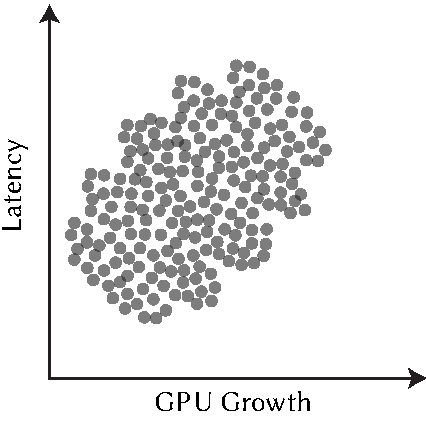
\includegraphics[width=0.45\linewidth]{fig__intro_1.pdf}}~
%     \subfloat[Observations segregated on \swapmem]
%     {\label{fig:intro_b}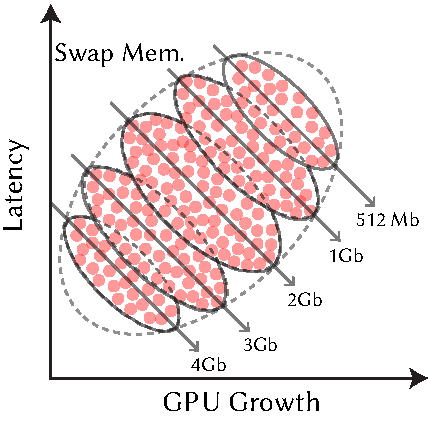
\includegraphics[width=0.45\linewidth]{fig__intro_2.pdf}}
%     \\[0.05em]
%     % \subfloat[Performance curves][Performance (Latency) curves]
%     % {\label{fig:intro_b}\includegraphics[width=0.68\linewidth]{fig__intro_b.pdf}}
%     \subfloat[][Causal Model]
%     {\label{fig:intro_c}\includegraphics[width=0.3\linewidth]{fig__intro_c.pdf}}\\[-1em]
%     \caption{\smallObservational data can sometimes lead to misleading inference. In \protectFig.~\ref{fig:intro_fig}a, the data (incorrectly) shows that high \gpugrowth leads to high latency. In \protectFig.~\ref{fig:intro_fig}b, the trend is reversed when the same data is segregated by \swapmem.}
%     \label{fig:intro_fig}
% \end{figure}

% Consequently, identifying the root cause of performance faults is notoriously difficult~\cite{gunawi2018fail} with as much as 99\% of them going unnoticed or unreported for extended durations~\cite{99ofmisc75:online}. This has tremendous monetary repercussions costing companies worldwide an estimated \$5 trillion in 2018 and 2019~\cite{Cloudmis78:online}. 


% ; or when they want to reason about performance in a different environment: \textit{``I’m trying to see how much faster the TX2 can classify images with TensorFlow than a Raspberry Pi model 3. My TensorFlow model was developed with transfer learning from the InceptionV3 CNN. My RPi takes about 20 seconds to classify an image, and to my surprise, the TX2 also takes about 20 seconds.~\cite{slowimag79:online}''}  
% \rayb{There are too many examples, we can reduce them to 1/2}
% Often developers are just curious to know whether an issue is arising due to misconfiguration, such as ~``\textit{I saw the latency is over 100ms, I am wondering if there is something misconfiguration or problems?~\cite{curious_issue:online}}.'' 
% The sheer number of modalities of software deployment is so large that exhaustively testing every conceivable software and hardware configuration is impossible!. 
% Crucially, these exchanges provoke other unanswered questions, such as ~``\textit{what would be the effect of changing another configuration `X'?~\cite{slowimag79:online}}.'' 

% Therefore, we seek methods that can \emph{identify, explain, and fix} the root cause of non-functional faults early in a principled fashion.


% \noindent\textbf{Existing work.}~
% Much recent work has focused on configuration optimization, which are approaches aimed at finding a configuration that optimizes a performance objective~\cite{wu2015deep, yigitbasi2013towards,siegmund2015performance, nair2018faster, filieri2015automated}. Finding the optimum configuration using push-button optimization approaches is not applicable here because they do not give us any information about the underlying interactions between the faulty configuration options that caused the non-functional fault. This information is sought after by developers seeking to address these non-functional faults~\cite{reddy2016fault, thung2012empirical}. 

\noindent\textbf{Existing works and gap.} Understanding the performance behavior of configurable systems can enable (i) performance debugging~\cite{SGAK:ESECFSE15,GSKA:SPPEXA}, (ii) performance tuning~\cite{H:CACM,SHM:LIO,H:AS,VPGFC:ICPE17,HPHL:ICSE15,WWHJK:GECCO15,NMSA:Arxive17,MARC:SPLC13,ORGC:SPLC14}, and (iii) architecture adaptation~\cite{JGAP:CSMR13,ABDD:VISSOFT13,KK:WSR16,JVKSK:SEAMS17,HSCMAR:SIGPLAN,FHM:FSE15,EEM:TSE,EEM:FSE10}. 
A common strategy is to build performance influence models such as regression models that explain the influence of individual options and their interactions~\cite{SGAK:ESECFSE15,VPGFC:ICPE17,GCASW:ASE13,pereira2019learning}. These approaches are adept at inferring the correlations between configuration options and performance objectives, however, as illustrated in~\fig{intro_fig} performance influence models suffer from several shortcomings (detailed in \S\ref{sec:motivation}): (i) they become ~\emph{unreliable in unseen environments} and (ii) ~\emph{produce incorrect explanations}.

% $f(c)=\beta_0+\Sigma_{i}{\phi(o_i)}+\Sigma_{i..j}{\phi(o_i..o_j)}$
% they lack the mathematical language to express \textit{how} the configuration options affect performance objectives. Without this, we risk drawing misleading conclusions. They also require significant time to gather the training samples, which grows exponentially with the number of configurations~\cite{kanellis2020too,xu2015hey}.  

% Prior work focuses on constructing performance influence models using machine learning or optimization methods~\cite{wu2015deep, yigitbasi2013towards, zhang2015performance,siegmund2015performance, nair2018faster, filieri2015automated, iqbal2020flexibo, jamshidi2016uncertainty}. These techniques cannot be used to diagnose and repair non-functional faults. There are several reasons for this. Firstly, these are usually pushbutton approaches that provide a one-size-fits-all optimal configuration that is very sensitive to minor changes to the system (\eg, slightly different workloads)~\cite{}. Secondly, they are adept at describing \textit{if} certain configuration options influence performance, however, they lack the mathematical language to express \textit{how} or \textit{why} the configuration options affect performance, without this, we risk drawing misleading conclusions. Lastly; they require significant time to gather the necessary measurements, and this grows exponentially with the number of configurations~\cite{}.  

% \noindent\textbf{Limitations of existing work.}~
% In \fig{intro_fig}, we present an example to help illustrate the limitations with current techniques. Here, the observational data gathered so far indicates that \gpugrowth is positively correlated with increased latency (as in Fig.~\ref{fig:intro_fig}a). An ML model built on this data will, with high confidence, predict that larger \gpugrowth leads to larger latency. However, this is counter-intuitive because higher \gpugrowth should, in theory, reduce latency not increase it. When we segregate the same data on \swapmem (as in~Fig.~\ref{fig:intro_fig}b), we see that there is indeed a general trend downward for latency, \ie, within each group of \swapmem, as \gpugrowth increases the latency decreases.
% We expect this because \gpugrowth controls how much memory the GPU can ``borrow'' from the \swapmem. Depending on resource pressure imposed by other host processes, a resource manager may arbitrarily re-allocate some \swapmem; this means the GPU borrows proportionately more/less swap memory thereby affecting the latency correspondingly. This is reflected by the data in Fig.~\ref{fig:intro_fig}b. If the ML-based model were to consult the available data (from Fig.~\ref{fig:intro_fig}a) unaware of such underlying factors, these models would be incorrect.
% With thousands of configurations, inferring such nuanced information from optimization or ML-based approaches would require a considerable amount of measurements and extensive domain expertise which can be impractical, if not impossible, to possess in practice.

% When we measure the latency by varying the \swapmem (and keeping \gpugrowth fixed), we observe that the latency vs. \swapmem curve changes minimally. When we double the \gpugrowth from $33\%$ to $66\%$, we observe a similar trend (Fig.~\ref{fig:intro_fig}b, top row). Conversely, when we increase \gpugrowth (under fixed \swapmem), we observe a sharp decline in latency. When the \swapmem is doubled from $2Gb$ to $4Gb$, the improvement in latency is more pronounced (Fig.~\ref{fig:intro_fig}b, bottom row). 

% Merely changing \swapmem would not affect latency without also changing \gpugrowth accordingly. 
% Further, external factors, \eg, other host processes, may affect both these configuration options. 
% Current methods do not allow us to understand these relationships. 
% 

% Therefore, to alleviate developers' burden, it is important to develop better methods to \emph{identify the root cause} of non-functional faults and \emph{fix} them early and in a principled way. % can be quite useful for software developers and system administrators.


% Statistical methods rely on simple ``correlation'' to draw their conclusions; these are heavily biased by the amount of available data resulting in a large number of false positives~\cite{}. \shariar{better example}For instance, correlation-based methods may highlight that certain \textit{scheduler policies} are correlated with high latency, however, they do not inform us if changing the scheduler policy alone can \textit{cause} the latency to improve. % can be quite useful for software developers and system administrators.

\noindent\textbf{Our approach.}~
Based on the several experimental pieces of evidence presented in the following sections, this paper proposes \ourapproach--a methodology that enables reasoning about configurable system performance with causal inference and counterfactual reasoning. \ourapproach first recovers the underlying causal structure from performance data. The causal performance model %instead of a performance model that has been learned using the mainstream regression-based approaches, 
allows users to (i)~identify the root causes of performance faults, (ii)~estimate the causal effects of various configurable parameters on the performance objectives, and (iii)~prescribe candidate configurations to fix the performance fault or optimize system performance. 
% 
% we propose the use of causal models~\cite{pearl2000models, pearl2009causality} to express the complex interactions between the configurations and the performance objectives with a rich graphical representation. Then, using counterfactual reasoning~\cite{pearl2011algorithmization} we identify the root cause of non-functional faults and prescribe repairs to fix the misconfigured options.
% 
% The causal model would also highlight that other hidden factors (\eg, other processes running on the host) may affect the configurations (shown by \circled{?} in Fig.~\ref{fig:intro_fig}c). 
% 
% To this end, 
% 

% For example, in~\fig{intro_fig}, \tool constructs a \textit{causal model} from observational data (as in Fig.~\ref{fig:intro_fig}c). This causal model indicates that \gpugrowth indirectly influences latency (via a \swapmem) and that the configuration options may be affected by certain other factors, \eg, resource manager allocating resources for other processes running on the host. \tool uses counterfactual questions such as, ``what is the effect of \gpugrowth on latency if the available \swapmem was 2Gb?'' to diagnose the faults and recommend changes to the configuration options to mitigate these faults. 


% \noindent\textbf{Evaluation.}~
% We evaluated \ourapproach in terms of its \emph{effectiveness, sample efficiency}, and \emph{scalability} and compared with state-of-the-art performance debugging and optimization using 5 real-world highly configurable systems (three machine learning systems, a video encoder, and a database system) deployed on 3 architecturally different NVIDIA Jetson devices. 

% We compare \ourapproach with state-of-the-art configuration optimization and ML-based performance debugging approaches. Overall, we find that \ourapproach is (at most) $13\times$ faster with $13\%$ better accuracy and $32\%$ higher gain than the next best ML-based approaches for single-objective faults. Compared to single-objective optimization approaches, \ourapproach can find repairs to misconfigurations $9\times$ faster while performing as well as (or better than) the best configuration discovered by the optimization techniques. Further, \ourapproach can find effective repairs for faults in multiple performance objectives (\ie, latency and energy consumption) with accuracy and gain as high as $16\%$ and $36\%$, respectively, than other ML-based performance debugging methods. Compared to multi-objective optimization approaches, \ourapproach can find repairs $5\times$ faster while having similar performance gain. Finally, with a case study, we demonstrate that \ourapproach finds $14\%$ better repairs than the experts' advice in 24 minutes.

% \tool would alleviate developers' burden, it is important to develop better methods to \emph{identify the root cause} of non-functional faults and \emph{fix} them early and in a principled way.
% If the prescribed repairs do not result in satisfactory performance improvement, \tool updates the causal model with new observations and repeats the above steps until the performance objective has been met. 

% Advise against the use of optimization:
%  - Don't want the global optima, but the original configuration with the smallest change to reach the performance objective. 
% - It does not give us any information on the underlying causality of the system. The explainability/expressiveness is lost -- we won't know how/why a certain change is useful. 
% Our work is tangentially related to other work on performance modeling and optimization of highly configurable systems using machine learning and optimization \cite{wu2015deep, yigitbasi2013towards, zhang2015performance,siegmund2015performance, nair2018faster, filieri2015automated, iqbal2020flexibo, jamshidi2016uncertainty}. These methods are designed as push-button solutions to offer a near-optimal configuration, they do not offer Here we essentially tackle a different problem---that of finding the root causes of an already observed non-functional fault and finding a fix for it instead of finding an optimization.

% , static and dynamic software analysis \cite{kim2013splat, meinicke2016essential, velez2019configcrusher, abal2018variability, nguyen2016igen}, or sampling techniques \cite{sarkar2015cost, siegmund2015performance, guo2013variability, jamshidi2018learning}.

% % \bi[leftmargin=*]
%     \noindent \textbf{Technique.} Our approach is the first to exploit causal inference and counterfactual reasoning to reason about the root causes for non-functional faults and offer repairs to fix them. 
%     % Our approach achieves this without actually performing any intervention (i.e., changing the configuration and deploying the system with the new configurations). This is unlike statistical debugging where we cannot reason about changes unless we have seen several failures to create discriminative models.

%     \noindent\textbf{Tool.} We propose \tool, a fully automated performance debugging approach that localizes the root causes of non-functional faults and fixes them. We show that \tool can handle faults in multiple performance objectives simultaneously. \tool is quite robust in that it can accommodate changes to software properties such as varying workloads. %We can reuse \tool to reason about non-functional faults in environments where we cannot collect new observations or we have only very few observational data. 

%     \noindent \textbf{Real-world Evaluation.} We evaluate \tool with 5 real-world highly configurable systems and it was able to identify the root causes and explain how the root causes (configuration options and interactions) triggered the fault, much more accurately with much less false negative compared with statistical debugging and the most popular heuristic approach in practice.
% % \ei



% \red{  Optimization tells us to configure under a certain way until the budget is finished. Need to collect new data to refine our estimate (bayesian opt) }
% \red{Analytical models require understanding and modeling of the system internal, which is impossible or expensive + data}
\begin{figure}[tp!]
    \centering
    \includegraphics*[width=\linewidth]{DeepStream-Arch.pdf}
    \caption{\small{\textsc{Deepstream}: An example of a highly-configurable composed system, a big data analytics pipeline system, with several configurable components: (i) Video Decoder performs video encoding/decoding with different formats; (ii) Stream Muxer accepts input streams and converts them to sequential batch frames; (iii) Primary Detector transforms the input frames based on input NN requirements and makes model inference to detect objects; (iv) Object Tracker supports multi-object tracking; (v) Secondary Classifier improves performance by avoiding re-inferencing.}}
    \label{fig:deepstream_pipeline}
    \vspace{-4mm}
\end{figure}


% \red{In eqs.~\ref{eq:do} and~\ref{eq:ace}, $\mathbb{E}(Y~|~do(X=x))$ is \textit{not} the same as the ordinary conditional distribution $\mathbb{E}\left(Y~|~X=x\right)$. This is because $\mathbb{E}\left(Y~|~X=x\right)$ takes the original population, as is, and filters it gets the sub-population where $X=x$. If $X=x$ does not exist in the population, the value of $\mathbb{E}\left(Y~|~X=x\right)$ would be misleading. In contrast, $\mathbb{E}\left(Y~|~\mathit{do}\left(X=x\right)\right)$ uses do-calculus rules~\cite{} to infer the value of distribution even when $X=x$ has never been encountered before. }
\noindent\textbf{Contributions.}~Our contributions are as follows:
\begin{itemize}
    \item We propose \ourapproach (\S\ref{sec:methodology}), a novel approach that allows causal reasoning about system performance.
    % causal diagnostics, and fault mitigation tool that identifies the root causes of non-functional faults and recommends repairs to resolve non-functional faults.% using a novel entropy-based causal structure discovery followed by causal effect estimation and counterfactual reasoning.
    \item We \emph{have conducted a thorough evaluation} of \ourapproach in a controlled case study (\S\ref{sec:casestudy}) as well as real-world large-scale experiments. In particular, we evaluated \emph{effectiveness} (\S\ref{sec:effectiveness}), \emph{transferability} (\S\ref{sec:transfer}), and \emph{scalability} (\S\ref{sec:scalability}) by comparing \ourapproach with: (i)~state-of-the-art performance debugging approaches, including \textsc{CBI}~\cite{song2014statistical}, \textsc{DD}~\cite{artho2011iterative}, \textsc{EnCore}~\cite{zhang2014encore}, and \textsc{BugDoc}~\cite{lourencco2020bugdoc} and (ii)~performance optimization techniques, including \textsc{SMAC}~\cite{hutter2011sequential} and \textsc{PESMO} \cite{hernandez2016predictive}. The evaluations were conducted on six real-world highly configurable systems, including a video analytic pipeline, \textsc{Deepstream}~\cite{DeepStream}, three deep learning-based systems, \textsc{Xception} \cite{chollet2017xception}, \textsc{Deepspeech}~\cite{hannun2014deep}, and \textsc{BERT}~\cite{devlin2018bert}, a video encoder, X264~\cite{x264}, and a database engine, SQLite~\cite{SQLite}, deployed on \textsc{NVIDIA Jetson} hardware (\txone, \txtwo, and \xavier). \item In addition to sample efficiency and accuracy of \ourapproach in finding root causes of performance issues, we show that the learned causal performance model is transferable across different workload and deployment environments. Finally, we demonstrate the scalability of \ourapproach to large systems consisting of 500 options and several trillion potential configurations.  
    % Our empirical results, conducted on 5 highly configurable systems deployed on 3 architecturally different hardware, \tool outperforms current state-of-the-art ML-based (Correlational, Association Rule Mining, Decision Tree, Regression Tree, Classification based approaches) diagnostics and optimization approaches in terms of efficacy (+16\% accuracy and +36\% gain) and speed (up to 13$\times$ faster). \tool was also adept at handling both single- and multi-objective performance faults. 
    % \item We offer a manually curated performance fault dataset (called Jetson Faults) and accompanying code required to reproduce our findings at 
    \item The artifacts and supplementary materials can be found at \href{github}{\color{blue!80} https://github.com/softsys4ai/unicorn}.
\end{itemize}   

